\chapter{Технологическая часть}

\section{Выбор среды и языка разработки}

\hspace{0.6cm} В качестве языка был выбран c\#, а вместе с ним и среда для разработки Visual Studio 2019. Так выбор был сделан в связи с:

\begin{itemize}
  \item Удобством удобством разработки, большим количеством вспомогательных функций (например, проверка синтаксиса);
  \item Наличием наличием диспетчера пакетов Nuget, позволяющего быстро добавлять необходимые расширения, без трат времени на долгий поиск и внедрение;
  \item Обозревателем обозревателем решений, позволяющим быстро переключаться между файлами в проекте.
\end{itemize}


\section{Используемые инструменты и технологии веб-приложения}

\hspace{0.6cm} В качестве фреймворка был выбран ASP.NET MVC. Причиной такого выбора стали:

\begin{itemize}
  \item Для данной задачи необходима реализации системы MVC, а данный фреймворк служит именно для этой цели;
  \item Наличие возможности реализовать Front-end вместе с Back-end используя HTML+CSS+C\#.
\end{itemize}

\hspace{0.6cm} Чтобы работать с базой данных через веб-приложение на C\# существует несколько вариантов:

\begin{itemize}
  \item Entity Framework — это решение для работы с базами данных, которое используется в программировании на языках семейства.NET. Оно позволяет взаимодействовать с СУБД с помощью сущностей (entity), а не таблиц. Также код с использованием EF пишется гораздо быстрее;
  \item MySQLConnector – динамическая библиотека предоставляющая возможность подключения и работы с MySql;
  \item MySQLData – динамическая библиотека предоставляющая возможность подключения и работы с MySql.
\end{itemize}

\hspace{0.6cm} Поскольку в качестве фреймворка был уже выбран ASP.net, удобнее выбрать динамическую библиотеку, поэтому была использована MySQLData. Для хостинга локального MySql сервера используется приложение MAMP.

\section{Реализация}

\hspace{0.6cm} При работе с базой устанавливается соединение с помощью строки подключения и функции динамической библиотеки MySQlData. Получение данных происходит после отправки запроса в СУБД. Запрос пишется на языке SQL. Работа с данными на серверной части осуществляется при помощи классов моделей, которые структурно совпадают с таблицами или с необходимым для нас выводом. Приложение при запуске начинает прослушивать порт 5001, по ip 127.0.0.1.

\section{Модель хранения}

На листингах \ref{list:user} и \ref{list:pet_info} представлены реализации классов user и pet\_info в программе.

\begin{lstlisting}[caption=класс User, label=list:user]
public int id { get; set; }
public string login { get; set; }
public string password { get; set; }
public string name { get; set; }
public string surname { get; set; }
public string role { get; set; }
\end{lstlisting}

\begin{lstlisting}[caption=класс pet\_info, label=list:pet_info]
public int pet_id { get; set; }
public string pet_type { get; set; }
public string name { get; set; } 
public int age { get; set; } 
public string color { get; set; } 
public int can_swim { get; set; } 
public int reproduce_ability { get; set; } 
public string gender { get; set; } 
public string pet_breed { get; set; } 
\end{lstlisting}

На листингах ниже представлены реализации запросов в базу данных.
Листинг \ref{list:GetUsers} – получение всех пользователей, листинг \ref{list:GetPetById} получение питомца по id.

\begin{lstlisting}[caption=функция получения всех пользователей, label=list:GetUsers]
public List<User> GetUsers()
{
    string sql = "SELECT * FROM `users`";

    cmd = new MySqlCommand();
    cmd.Connection = conn;
    cmd.CommandText = sql;

    var users = new List<User>();

    using (DbDataReader reader = cmd.ExecuteReader())
    {
        if (reader.HasRows)
        {
            while (reader.Read())
            {
                int userId = Convert.ToInt32(reader.GetValue(reader.GetOrdinal("user_id")));
                string login = reader.GetString(reader.GetOrdinal("login"));
                string password = reader.GetString(reader.GetOrdinal("password"));
                string name = reader.GetString(reader.GetOrdinal("name"));
                string surname = reader.GetString(reader.GetOrdinal("surname"));
                string role = reader.GetString(reader.GetOrdinal("role"));

                users.Add(new User(userId, login, password, name, surname, role));

            }
        return users;
        }
    }
    return users;
}
\end{lstlisting}

\begin{lstlisting}[caption=функция получения питомца по id, label=list:GetPetById]
public Pet GetPetById(int id)
{
    string sql = \"Select * from `pets` where pet_id = @id";

    cmd = new MySqlCommand();
    cmd.CommandText = sql;
    cmd.Connection = conn;
    cmd.Parameters.Add("@id", MySqlDbType.Int32).Value = id;
    
    var pet = new Pet();
    try
    {
        using (DbDataReader reader = cmd.ExecuteReader())
        {
            if (reader.HasRows)
            {
                while (reader.Read())
                {
                    pet.pet_id = Convert.ToInt32(reader.GetValue(reader.GetOrdinal("pet_id")));
                    pet.price = Convert.ToInt32(reader.GetValue(reader.GetOrdinal("price")));
                    pet.shop_id = Convert.ToInt32(reader.GetValue(reader.GetOrdinal("shop_id")));
                    pet.availability = reader.GetString(reader.GetOrdinal("availability"));
                    return pet;
                }
            }
        }
    }
    catch(Exception e)
    {
        Console.WriteLine("Error: " + e);
    }
    return null;
}
\end{lstlisting}

\newpage

\section{Интерфейс программы}

\hspace{0.6cm} Ниже представлен интерфейс веб-приложения.

\begin{figure}[ht!]
  \centering
  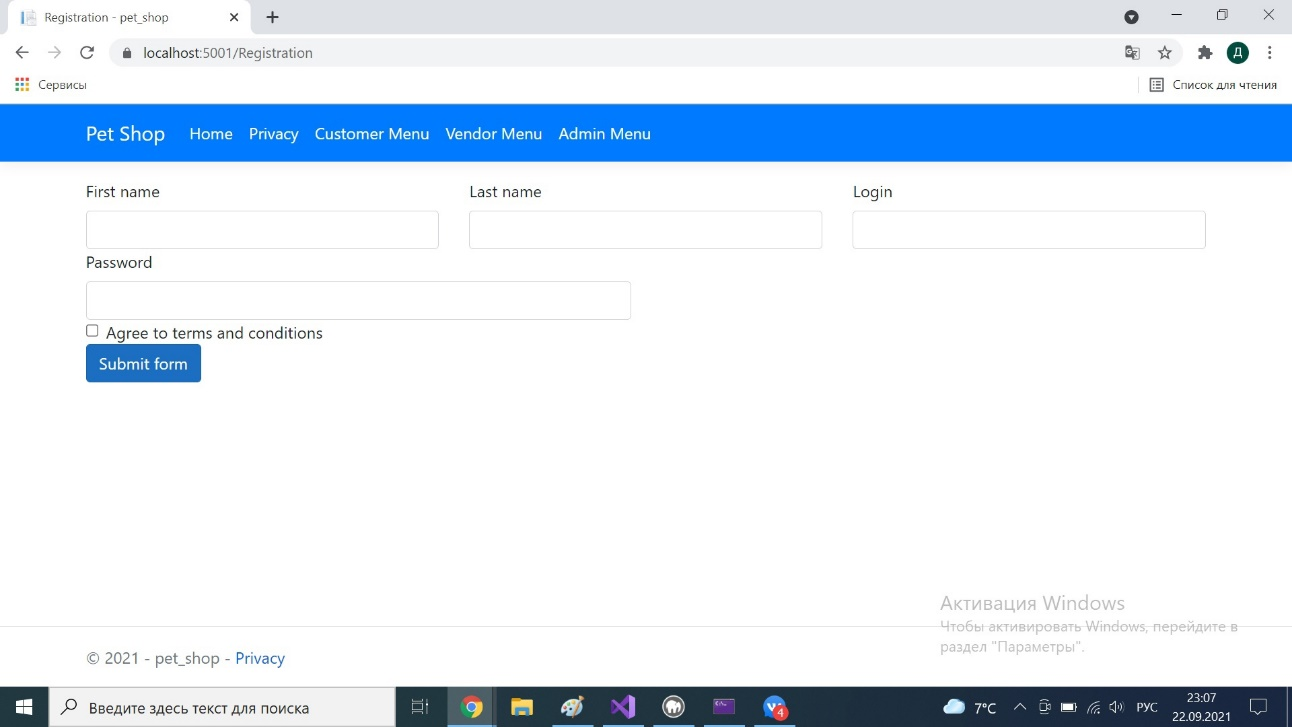
\includegraphics[scale=1]{img/interface1.png}
  \caption{Окно регистрации}
  \label{fig:interface1}
\end{figure}

\begin{figure}[ht!]
  \centering
  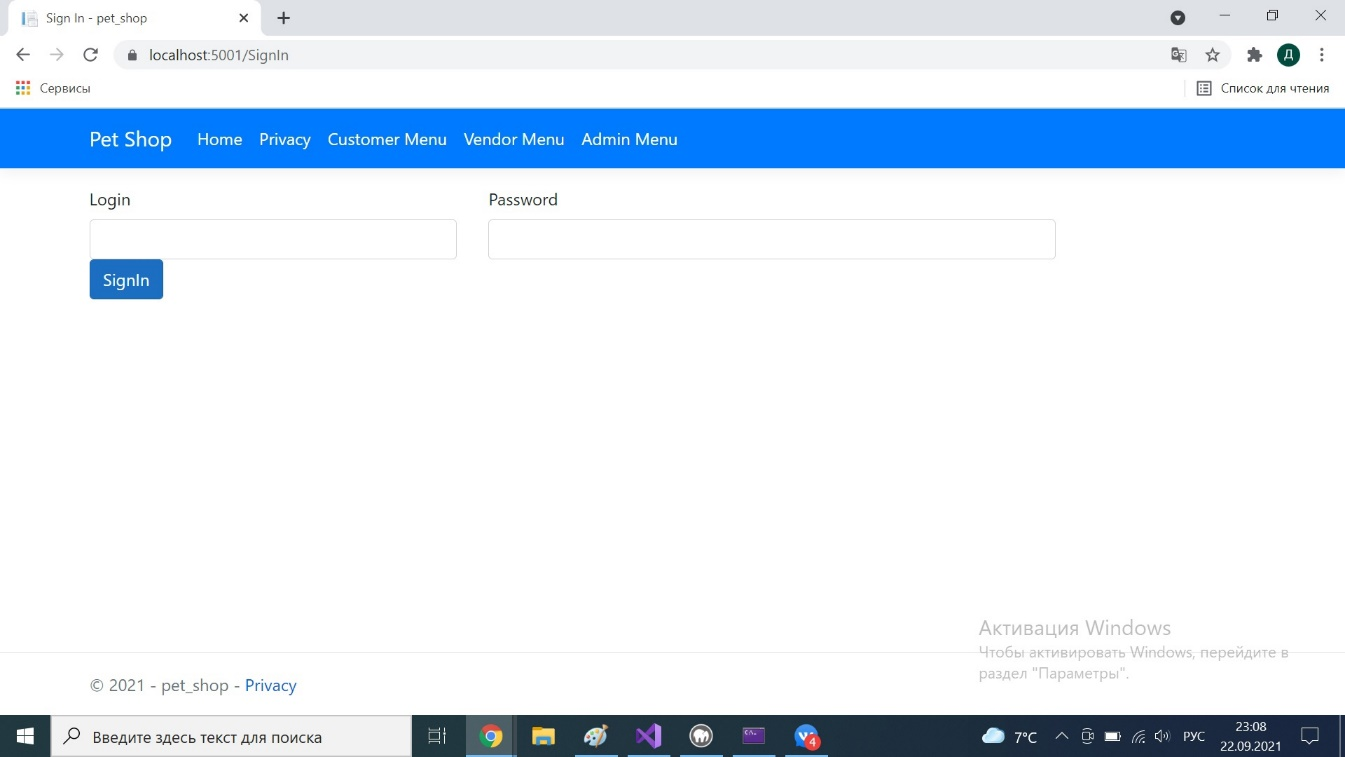
\includegraphics[scale=1]{img/interface2.png}
  \caption{Окно авторизации}
  \label{fig:interface2}
\end{figure}

\newpage

\begin{figure}[ht!]
  \centering
  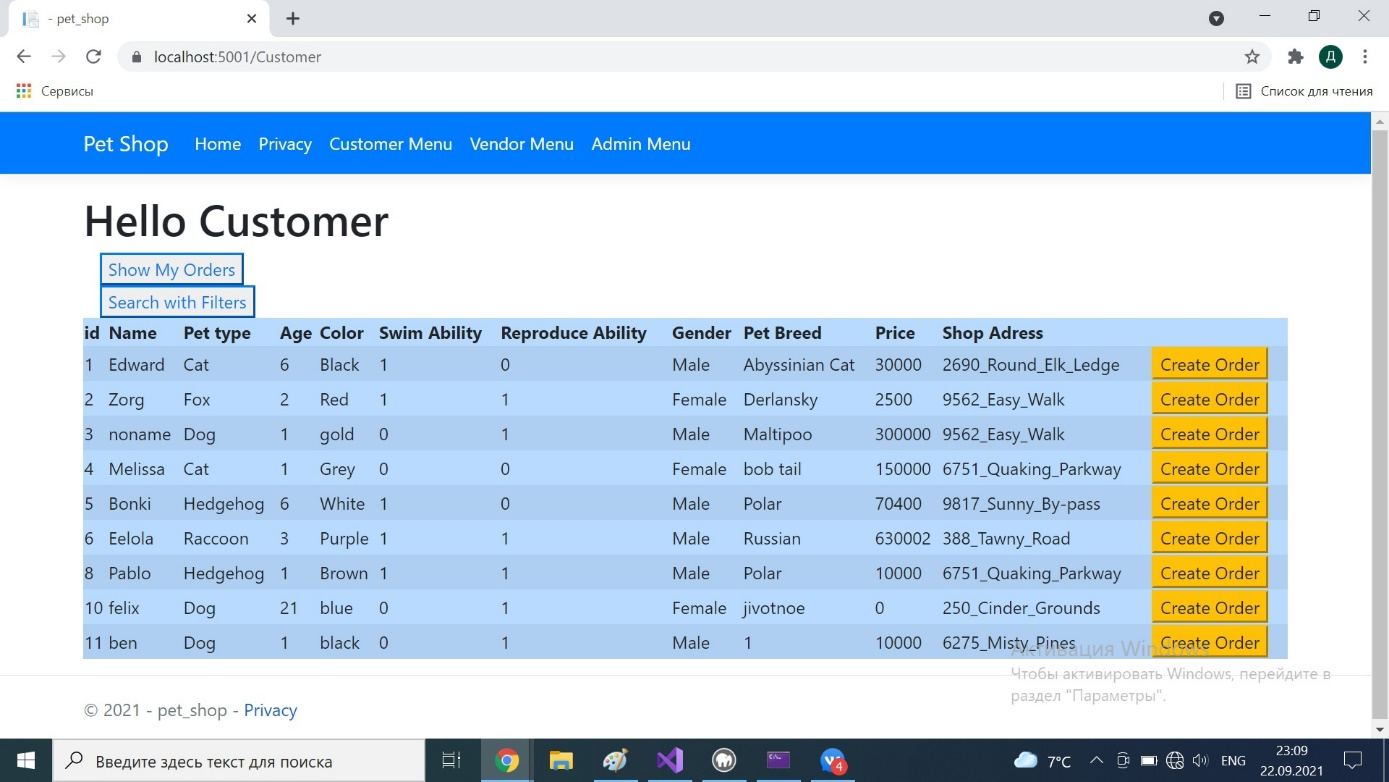
\includegraphics[scale=0.9]{img/interface3.png}
  \caption{Окно покупателя}
  \label{fig:interface3}
\end{figure}

В меню покупателя на рисунке \ref{fig:interface3} можно создавать заказы, а также просматривать доступные товары.

\begin{figure}[ht!]
  \centering
  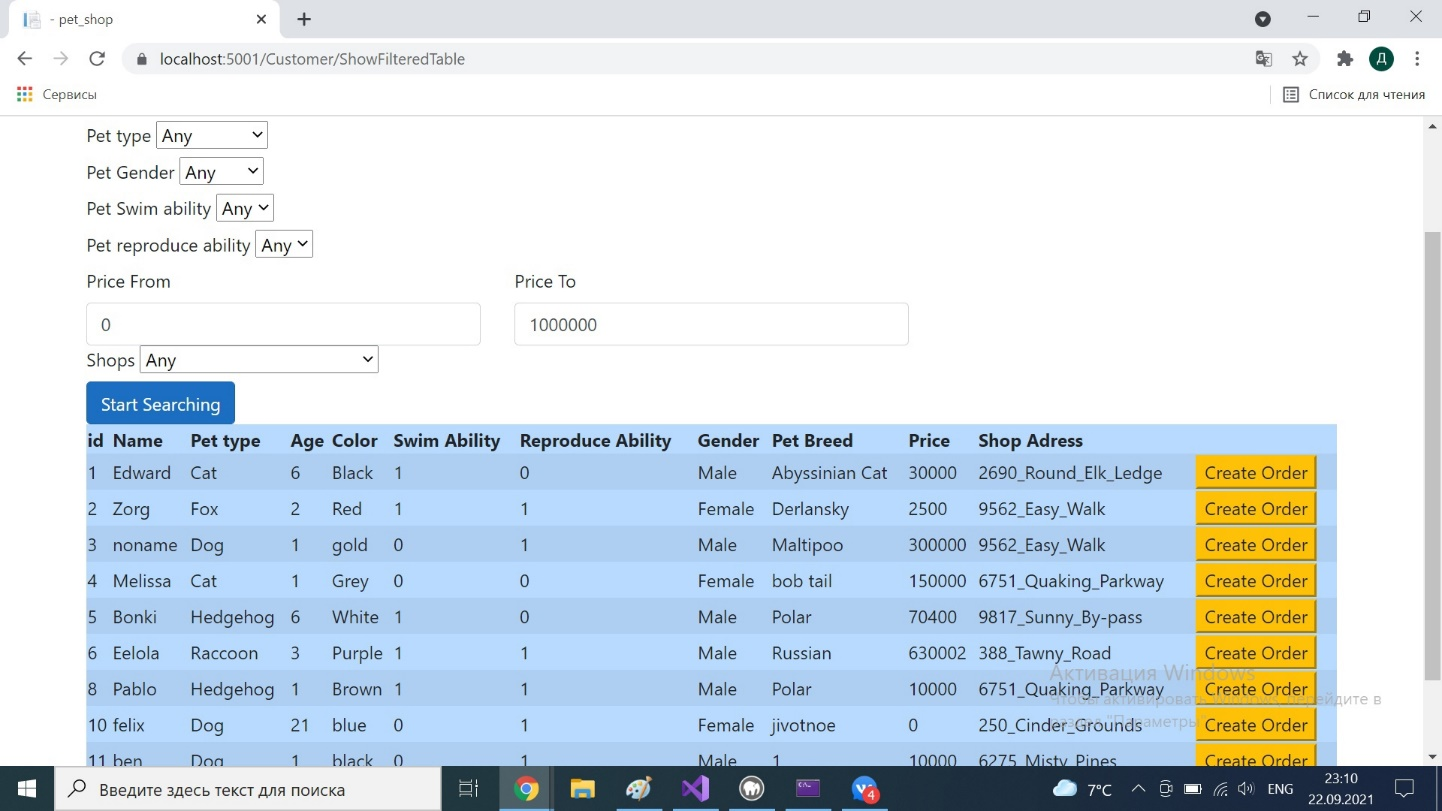
\includegraphics[scale=0.9]{img/interface4.png}
  \caption{Окно поиска товаров с фильтром}
  \label{fig:interface4}
\end{figure}

В окне, изображенном на рисунке \ref{fig:interface4}, можно просматривать товары и делать заказы, только с возможностью выбрать конкретные интересующие покупателя товары.

\newpage

\begin{figure}[ht!]
  \centering
  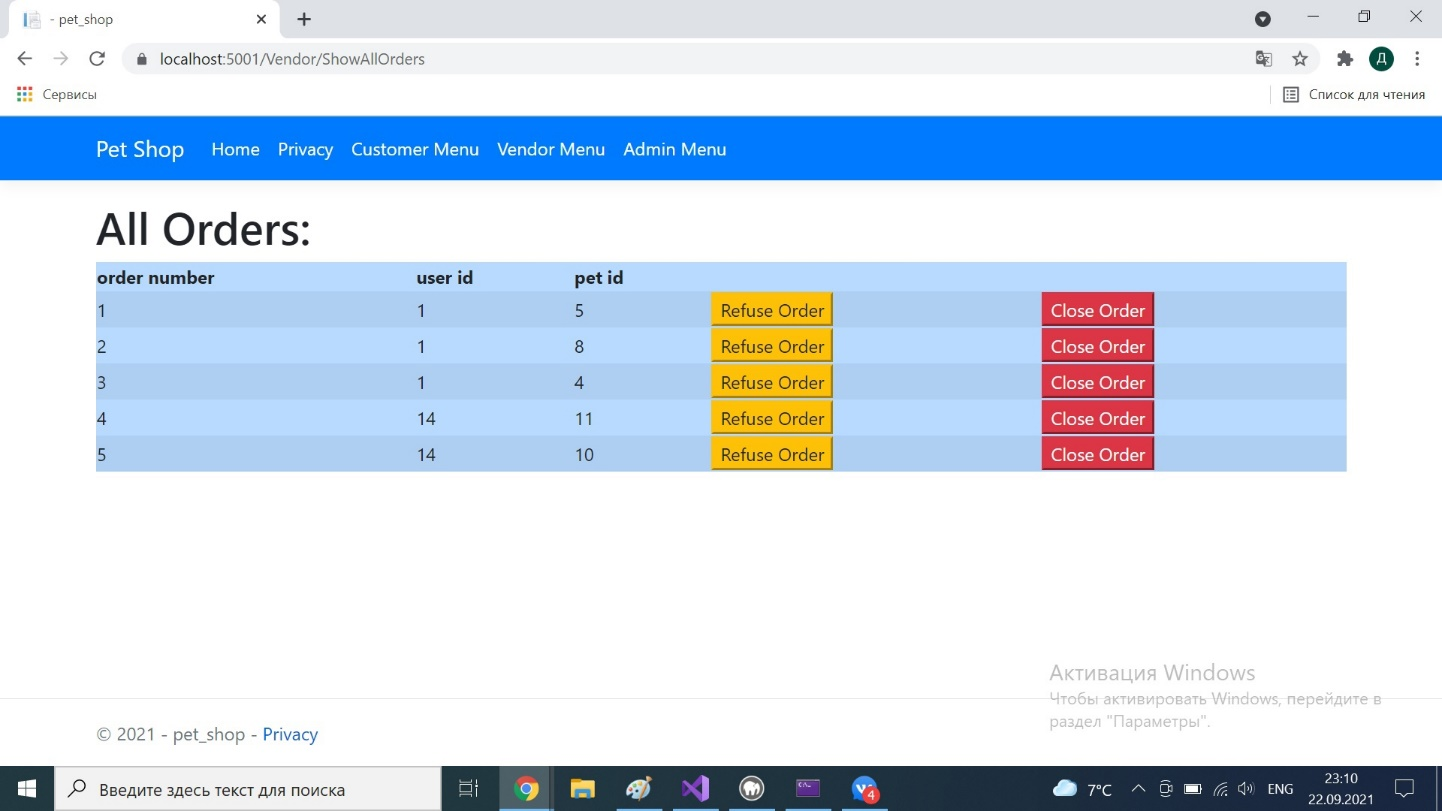
\includegraphics[scale=0.9]{img/interface5.png}
  \caption{Окно продавца}
  \label{fig:interface5}
\end{figure}

В окне продавца на рисунке \ref{fig:interface5} присутствуют все заказы. Есть возможность отклонить заказ, если покупатель не может сделать этого сам или закрытие заказа, что означает, что покупка питомца была совершена.

\begin{figure}[ht!]
  \centering
  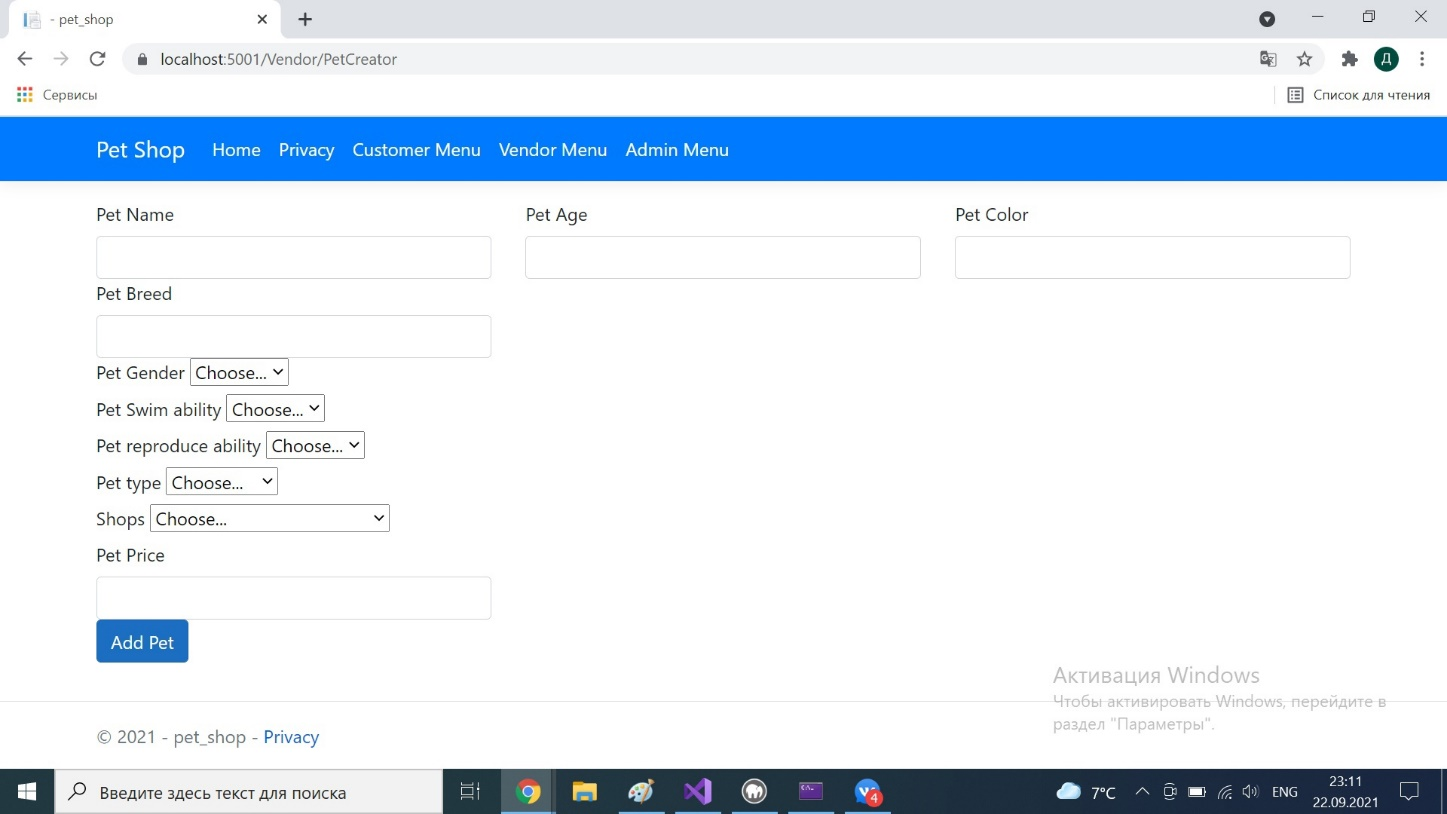
\includegraphics[scale=0.9]{img/interface6.png}
  \caption{Окно создания товара}
  \label{fig:interface6}
\end{figure}

В окне создания товара на рисунке \ref{fig:interface6} продавец может добавить новое животное в список доступных.

\newpage

\begin{figure}[ht!]
  \centering
  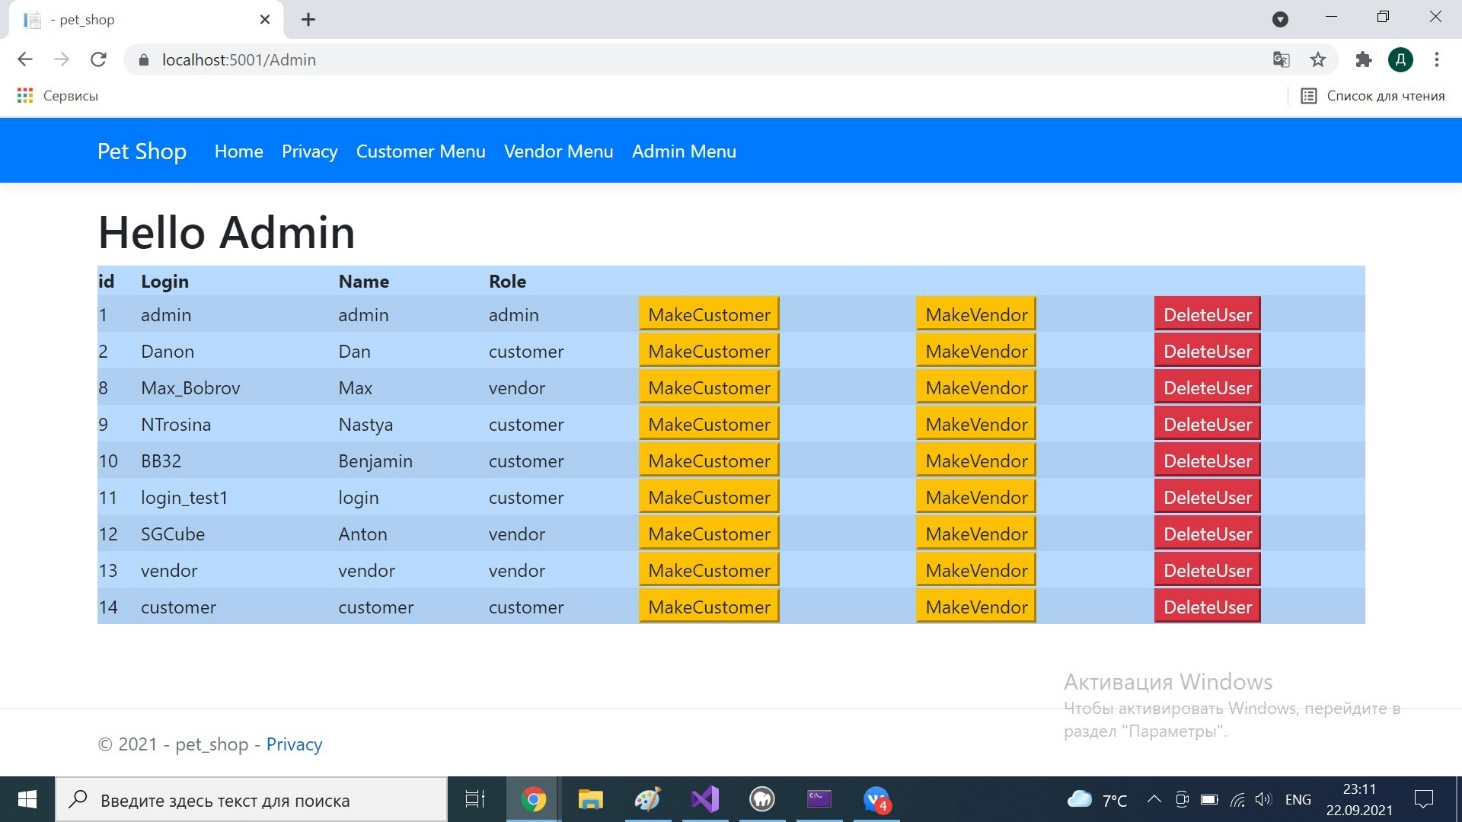
\includegraphics[scale=0.9]{img/interface7.png}
  \caption{Окно администратора}
  \label{fig:interface7}
\end{figure}

Администратор имеет возможность удалять пользователей, либо изменять их роли. В системе администратор зарегистрирован может быть только один.

\newpage

\section{Вывод}
В данном разделе были описаны выбранные средства, среда разработки, язык, СУБД, а также продемонстрирован интерфейс веб-приложения.
